\documentclass[twocolumn]{article}

\usepackage{graphicx}
\usepackage{amsmath}
\usepackage{url}
\usepackage{subfig}
\usepackage{algorithm}
\usepackage{algpseudocode}
\usepackage{booktabs}
\usepackage[sort&compress]{natbib}
\usepackage{setspace}

\begin{document}

\title{V4 Neural Network Model for Shape-based Feature Extraction and Object Discrimination}

\author{Hui Wei\footnote{Corresponding author} \and Zheng Dong
\footnote{Hui Wei and Zheng Dong are with the Laboratory of Cognitive Modeling and Algorithms, %
School of Computer Science, Fudan University, Shanghai, China. %
Corresponding author's email: weihui@fudan.edu.cn}}

\date{}

\maketitle

\begin{abstract}
Visual area V4 plays an important role in the neural mechanism of shape recognition.
V4 neurons exhibit selectivity for the orientation and curvature of boundary fragments.
In this paper, we propose a novel neural network model of V4 for shape-based feature extraction and other vision tasks.
The low-level layers of the model consist of computational units simulating simple cells and complex cells in the primary visual cortex.
These layers extract preliminary visual features including edges and orientations.
The V4 computational units calculate the entropy of the extracted features as a measure of visual saliency.
The features around salient points are then selected and encoded with a layer of Restricted Boltzmann Machine 
to generate an intermediate representation of object shapes.
The model is evaluated in shape distinction, feature detection, feature matching and object discrimination experiments.
The results demonstrate that this model generates discriminative local representation of object shapes.
It shows a successful attempt to construct a computation model of visual object recognition in the brain.
\end{abstract}

Keywords:
Neural network model, visual cortex, V4, shape selectivity, feature extraction, object recognition

\section{Introduction}

Understanding the content of images has always been a difficult task in image analysis due to the well known semantic gap \cite{smeulders2000}.
A high degree of abstraction is required to transform low-level pixel data into high-level knowledge of the images.
In an attempt to bridge this semantic gap, various methods have been proposed to extract features from the pixel representation of images.
However, humans and primates outperform any existing computer vision system with respect to almost any measure.
Though the neural mechanism of vision has not been fully revealed,
recent research on neuroscience do provide many inspiring discoveries which would help development of computer vision algorithms.
In this paper, we demonstrate a novel model of visual area V4 and its application to shape-based feature extraction and object discrimination.
Experimental results show that the proposed model exhibits similar shape selectivity to that of real V4 neurons
and it outperforms many existing methods in computer vision tasks including feature matching and object recognition. 

V4 lies in the middle of the ventral visual pathway \cite{ettlinger1990}, 
which is the neural stream involved with object recognition in the brain (\figurename~\ref{fig:1}).
It extracts the feature of contour conformation, which represents a middle level abstraction of visual information in the brain.
Lower levels (V1 and V2) extract features such as edges and orientations \cite{hubel1962}.
Higher levels (inferior temporal cortex) comprehend concepts of complex objects like faces and body parts \cite{bell2009}.
As an intermediate stage, V4 plays a crucial role in transforming low-level orientation signals into complex object representations.

\begin{figure}[!t]
\centerline{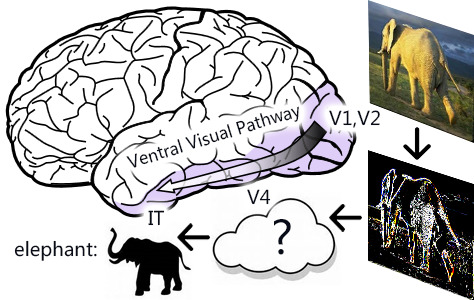
\includegraphics[width=0.8\linewidth]{images/fig1.jpg}} 
\caption{V4 is an intermediate stage in visual recognition.}
\label{fig:1}
\end{figure}

In this paper, we propose a multilayer neural network model which imitates the neural mechanism of visual area V4 in the ventral visual pathway.
Different stages of the neural pathway in the visual cortex are explicitly mapped to different layers of the neural network model.
In this feed-forward network, features are extracted hierarchically from input images.
High-level local image features emerge in the output layer of the network. 
The features encode local structures of object shapes in a way which closely resembles the mechanism of the cortex.
With a limited number of training images, the model can learn to distinguish between different categories of objects.
Moreover, this multilayer neural network shows a successful attempt to integrate different stages of visual processing in the brain. 
It provides an extensible framework so that future findings in cortical mechanisms can be adopted and applied to computer vision tasks.

We briefly introduce some related work on V4 models in section~\ref{sec:2}.
In section~\ref{sec:3}, we give the detailed description of the proposed model.
It is capable of locating salient points and generating discriminative local shape features around salient points.
In section~\ref{sec:4}, we show several experiments in which we evaluate the model.
The model is compared with real V4 neurons in a shape distinction experiment.
The features extracted by the model are applied to various computer vision tasks.
The discussion and conclusion is summarized in section~\ref{sec:5}.

\section{Related work}\label{sec:2}

In this section, we briefly review some existing models of V4 and other related models.

V4 neurons have been examine with different varieties of visual stimuli, including light bars, sinusoidal gratings~(\figurename~\ref{fig:2a}),
non-Cartesian gratings~(\figurename~\ref{fig:2b}), and closed shapes~(\figurename~\ref{fig:2c}) \cite{gallant1996,pasupathy2001}.
They generally prefer complex features to simple features such as bars and sinusoidal gratings \cite{gallant1996}.
Most V4 neurons are tuned for the curvature and orientation of boundary fragments \cite{pasupathy2001}.
Therefore, unlike neurons in V1, V4 neurons can not be modeled with linear filters.

\begin{figure}[!t]
\centering
\subfloat[]{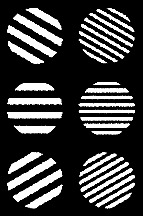
\includegraphics[width=0.18\linewidth]{images/fig2a.jpg}\label{fig:2a}}\hfil
\subfloat[]{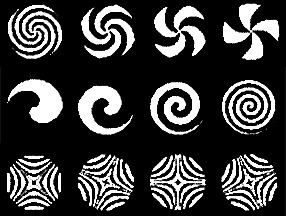
\includegraphics[width=0.36\linewidth]{images/fig2b.jpg}\label{fig:2b}}\hfil
\subfloat[]{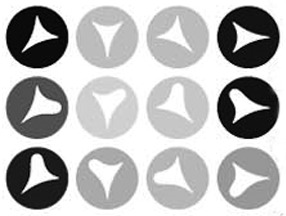
\includegraphics[width=0.36\linewidth]{images/fig2c.jpg}\label{fig:2c}}
\caption{Shapes to examine V4 selectivity.
(a) Sinusoidal gratings. (b) Non-Cartesian gratings. (c) Closed shapes.}
\label{fig:2}
\end{figure}

Several models have been proposed for V4 neurons.
We briefly introduce the SRF model \cite{david2006} and the HMAX model \cite{cadieu2007}.
The spectral receptive field (SRF) \cite{david2006} describes properties of V4 receptive field in terms of the orientation and spatial frequency spectrum.
This model is powerful in describing the shape selectivity of V4 neurons.
However, it does not provide any computational or neural mechanism to achieve V4 selectivity via spectral receptive field.
The HMAX model was first proposed in \cite{riesenhuber1999} as a generic model for object recognition in the visual cortex.
It models the visual cortex as a hierarchical architecture consisting of cascaded linear filters and non-linear maximum pooling operations.
It has been also adopted as a model for V4 shape selectivity and invariance \cite{cadieu2007}.
Training this model is an NP-complete problem. 
The authors used a greedy algorithm to obtain approximated solutions but they did not provide any biological evidence for the algorithm. 

The deep learning model also draws inspiration from the layered structure of the cortex \cite{bengio2009}.
It learns representations of data through stacked layers of Restricted Boltzmann Machines (RBM).
When it is trained with natural images, 
the kernels of the data-connected layer resemble the pattern of the receptive field of neurons in the primary visual cortex.
By training many stacked layers of RBM, highly abstracted features can be extracted automatically from input images.
Therefore, with additional fine tuning, the deep model exhibits high performance in image classification \cite{krizhevsky2012}.
Our proposed model employs a similar multilayer structure but combines automatic feature extraction with artificial features.
This combined strategy allows our model to work on fewer training images.

\section{Multilayer neural network model}\label{sec:3}

The information processing in the visual cortex follows a hierarchical scheme.
Our model employs a similar hierarchical structure.
Different cortical areas along the neural pathway are explicitly mapped to different layers in our model. 
\figurename~\ref{fig:3} shows the architecture of our model.

\begin{figure}[!t]
\centerline{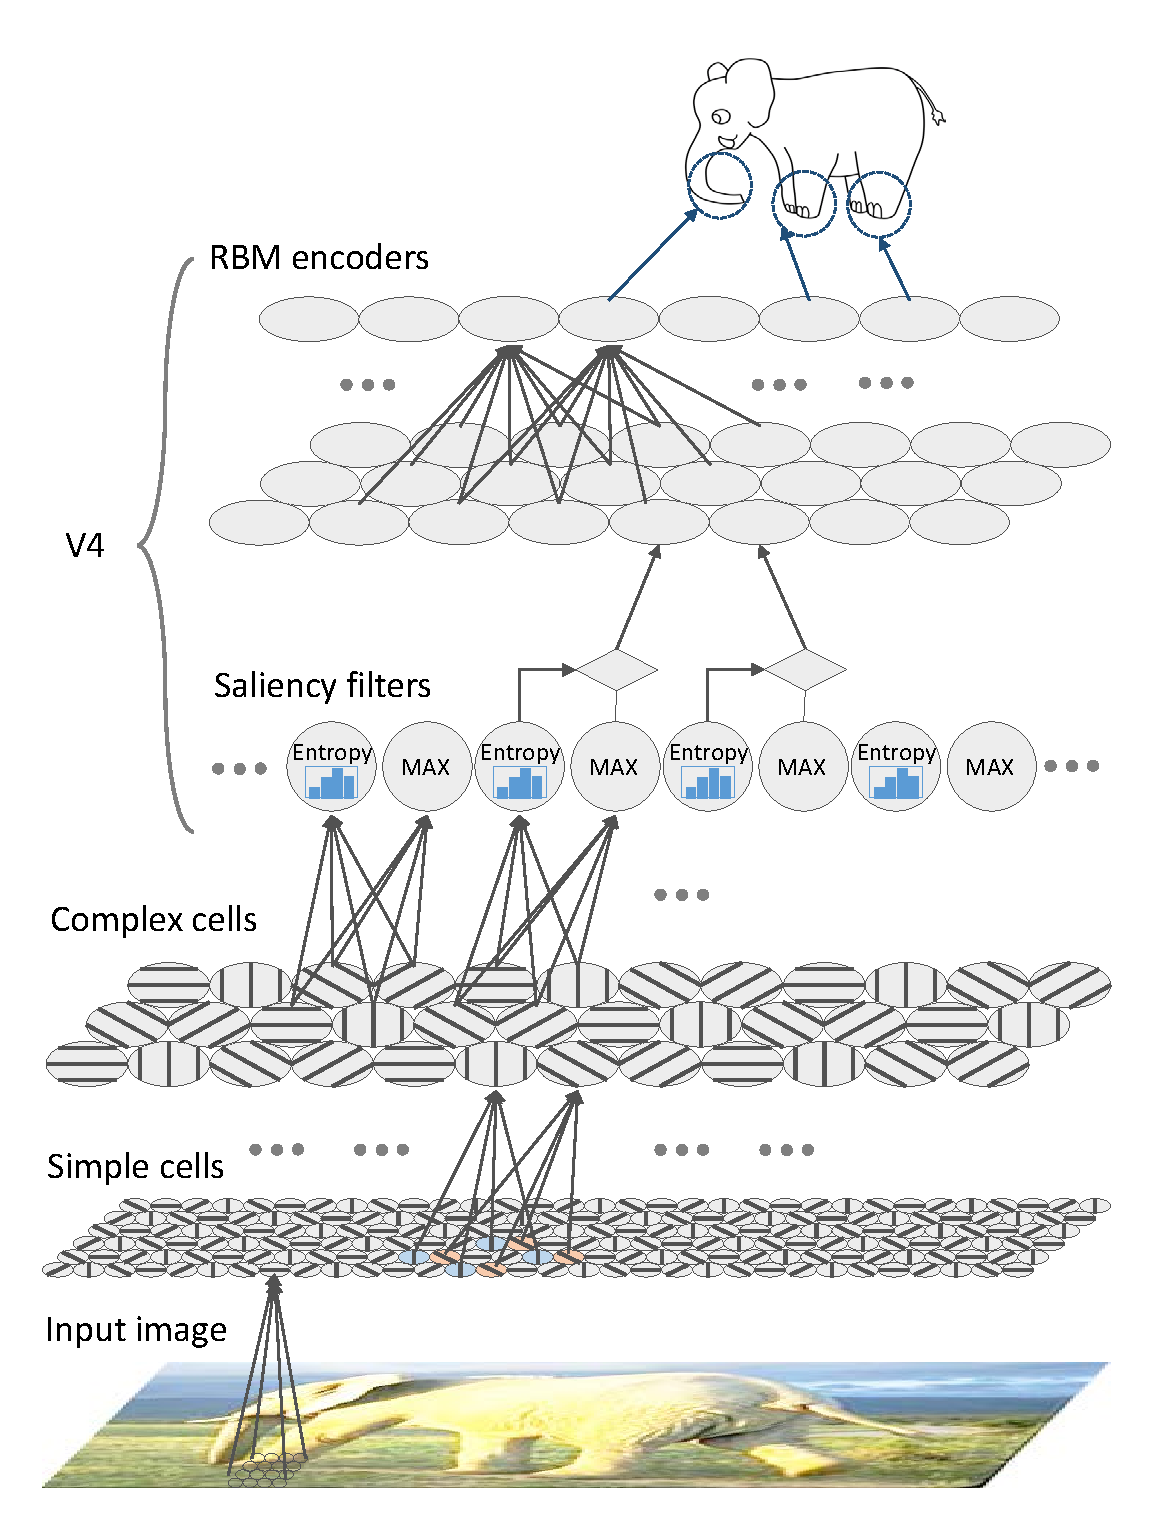
\includegraphics[width=\linewidth]{images/fig3.eps}} 
\caption{Multilayer neural network model of V4.}
\label{fig:3}
\end{figure}

\subsection{Layers of simple cells and complex cells}

According to the hierarchy of the visual cortex, area V4 receives input from the lower levels including area V1 and V2.
Neurons in V1 and V2 respond to local orientations.
They fall into two categories, simple cells and complex cells.
A simple cell is activated when an edge stimulus is presented in its receptive field with appropriate orientation and position.
Complex cells have larger receptive fields.
A stimulus is effective wherever it is placed in the complex receptive field, provided that the orientation is appropriate \cite{hubel1962}.

In our model, simple cells are modeled as Gabor functions,
\begin{equation}\label{equ:gabor}
g_{\theta}(x,y;\lambda,\sigma_s)
=\exp \left(-\frac{x'^2+y'^2}{2\sigma_s^2}\right)
\cos\frac{2\pi x'}{\lambda},
\end{equation}
where $x'=x\cos\theta+y\sin\theta$, $y'=-x\sin\theta+y\cos\theta$.
In the equation, $\lambda$ is the wavelength of the sinusoidal factor, 
$\theta$ represents the preferred orientation,
and $\sigma_s$ approximates the radius of the receptive fields.

Simple cells operates on raw image input. 
The output of simple cells with preferred orientation $\theta$ and scale $\sigma_s$ is the following convolution passed through a transfer function $\phi$,
\begin{equation}\label{equ:gabor}
S_{\theta,\sigma_s}(x,y)=\phi(I\otimes g_{\theta,\sigma_s}),
\end{equation}
where $I$ is an image and 
\begin{equation}\label{equ:gabor}
\phi(u)=\left\{\begin{array}{ll}
u & \text{if } u>0,\\
0 & \text{otherwise.}
\end{array}\right.
\end{equation}

Complex cells are modeled as Gaussian filters which take input from simple cells,
\begin{equation}
f(x,y;\sigma_c)=\frac{1}{2\pi\sigma_c^2}\exp\left(-\frac{x^2+y^2}{2\sigma_c^2}\right),
\end{equation}
where $\sigma_c$ represents the radius of the complex receptive fields.
The radius of complex receptive field is approximately twice as long as that of a simple cell.
We take this size because qualitatively the complex receptive fields are usually two to five times wider 
than the bars of gratings that stimulate them most effectively \cite{hubel1962}.
In this paper, we have $\sigma_c=2\sigma_s$.

Given $I(x,y)$ as some input image, the output of complex cells with the preferred orientation $\theta$ is defined as the following convolution.
\begin{equation}
C_{\theta}=S_{\theta}\otimes f.
\label{equ:complex}
\end{equation}

In the HMAX model \cite{riesenhuber1999} and the deep convolutional neural network \cite{krizhevsky2012}, pooling operation is an important step.
Pooling features over a local neighborhood can create invariance to small transformations of the input \cite{boureau2010}.
In our model, complex cells carry out similar function.
The operation can be viewed as a Gaussian-weighted average pooling.
We choose weighted average pooling because average pooling can be efficiently calculated with artificial neurons
and weighted average gives the complex cell's receptive field a smooth and circular boundary.  

\subsection{Saliency filters in V4 layer}

Visual attention involves selecting an interested region or selecting specific object features.
Area V4 shows selective attention based on spatial location \cite{desimone1995}.
The underlying neural mechanism is unknown.
V4 neurons exhibit preference for geometrically ordered stimuli \cite{sasaki2005}.
Therefore we use entropy (a measure of disorder) to measure the saliency of images.
The entropy is calculated according to the output of complex cells.
Given a point $(x,y)$, in the neighborhood of $(x,y)$,
a complex cell with preferred orientation $\theta$ has output value $C_{\theta}(x,y)$,
We suppose that the probability of a complex cell being activated is proportional to the output value.
The probability is thus defined as:
\begin{equation}
P(\theta)=\frac{1}{\sum_{\theta_i} C_{\theta_i}(x,y)}\cdot C_{\theta}(x,y).
\end{equation}
The entropy of the complex cell activity in this neighborhood is 
\begin{equation}
E=-\sum_{\theta} P(\theta) \log P(\theta).
\end{equation}

\figurename~\ref{fig:4} shows four image patches.
For each image patch, the output values of complex cells with different preferred orientations (from $0^\circ$ to $180^\circ$) are plotted in a bar chart.
The charts show the distribution of complex cell activities.
The entropy calculated accordingly indicates that patches composed of geometrically ordered structures have non-uniform distributions and thus low entropy values.
Therefore, we filter out regions with high entropy.

\begin{figure}[!t]
\centerline{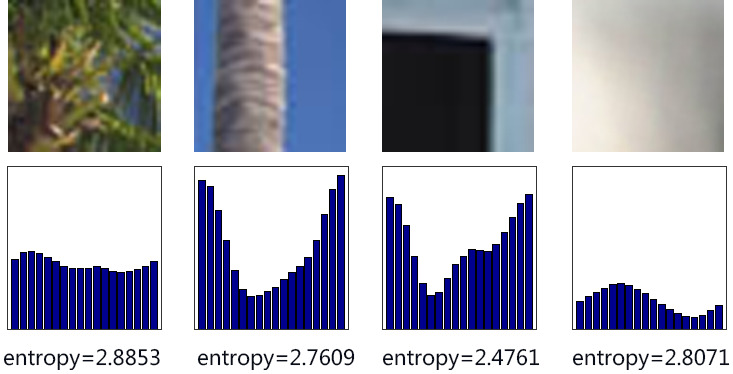
\includegraphics[width=0.8\linewidth]{images/fig4.jpg}} 
\caption{Entropy of image patches.
Bar charts in the second row show the output values of complex cells
with different preferred orientations (from $0^\circ$ to $180^\circ$).}
\label{fig:4}
\end{figure}

In addition to entropy, local competition also plays a role in attentional selection \cite{desimone1995}.
In our model, the saliency layer finds local maximums of complex cell output and filters out those points with high entropy values or low activities.
The algorithm is listed in Algorithm \ref{alg:1}.
In our experiment, the saliency filters take a threshold $t_E=2.8$ for the entropy
and a threshold $t_A=0.4$ for complex cell output value (or complex cell activity).
These values are roughly the median values of natural images.

\begin{algorithm}
  \caption{Saliency filter}
  \label{alg:1}
  \begin{algorithmic}[1]
    \Procedure{FindSalientPoint}{image $I$, scale $\sigma_c$, threshold $t_A,t_E$}
      \For{each orientation $\theta$}
        \State $C_{\theta}\leftarrow\phi(I\otimes g_{\theta})\otimes f_{\sigma_c}$
        \Comment{complex cell output}
      \EndFor
      \For{each point $(x,y)$ in image $I$}
        \State $C(x,y)\leftarrow\max_{\theta}C_{\theta}(x,y)$
        \State $E(x,y)\leftarrow$ entropy at point $(x,y)$
      \EndFor
      \State Divide image $I$ into patches of size $\sigma_c\times\sigma_c$
      \For{each patch $p$}
        \State $(\hat{x},\hat{y})\leftarrow\operatorname{argmax}_{(x,y)\in p}C(x,y)$
        \If{$C(\hat{x},\hat{y})>t_A$ and $E(\hat{x},\hat{y})<t_E$}
          \State Mark $(\hat{x},\hat{y})$ as a salient point
        \EndIf
      \EndFor
    \EndProcedure
  \end{algorithmic}
\end{algorithm}

\figurename~\ref{fig:5} shows the process of feature detection.
Saliency filters successfully filter out the trees and handwriting at the background of the images.
These regions have little shape features but the activity map of complex cells contains high values caused by a large amount of disordered edges. 
Disordered edges result in high entropy values because the distribution of complex cell activity over different orientations is near uniform.
Saliency filters filter out these regions by applying a threshold to the entropy map.

\begin{figure}[!t]
\centering
\subfloat[Car image]{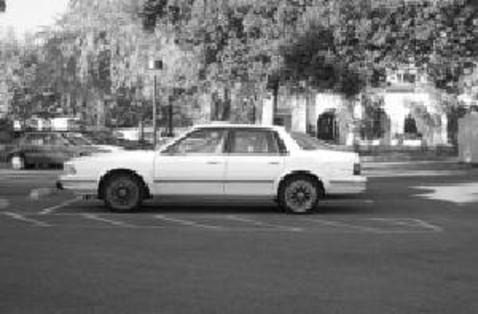
\includegraphics[width=0.32\linewidth]{images/fig5a.jpg}\label{fig:5a}}\hfil
\subfloat[Activity map]{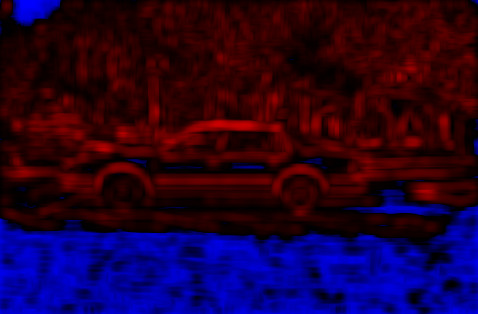
\includegraphics[width=0.32\linewidth]{images/fig5c.jpg}\label{fig:5b}}\hfil
\subfloat[Entropy map]{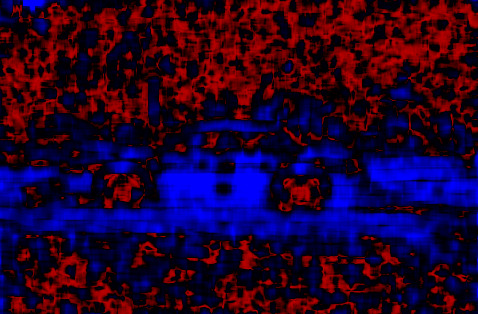
\includegraphics[width=0.32\linewidth]{images/fig5e.jpg}\label{fig:5c}}\\
\subfloat[Face image]{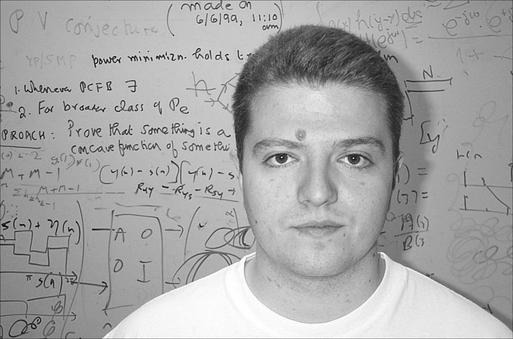
\includegraphics[width=0.32\linewidth]{images/fig5b.jpg}\label{fig:5d}}\hfil
\subfloat[Activity map]{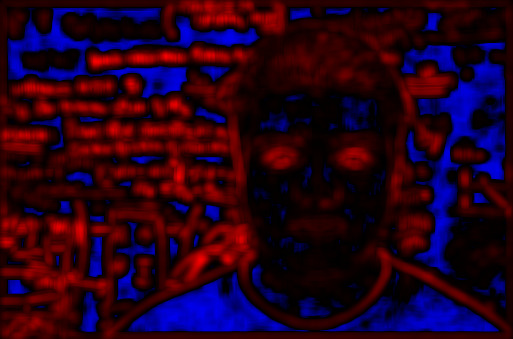
\includegraphics[width=0.32\linewidth]{images/fig5d.jpg}\label{fig:5e}}\hfil
\subfloat[Entropy map]{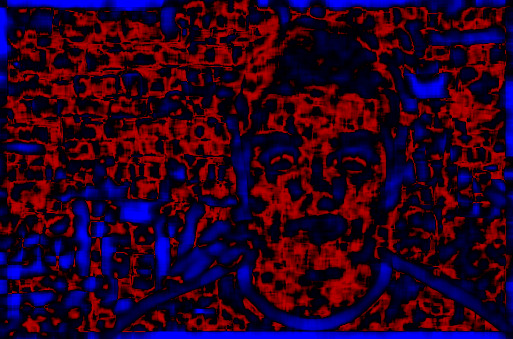
\includegraphics[width=0.32\linewidth]{images/fig5f.jpg}\label{fig:5f}}\\
\subfloat[Salient points]{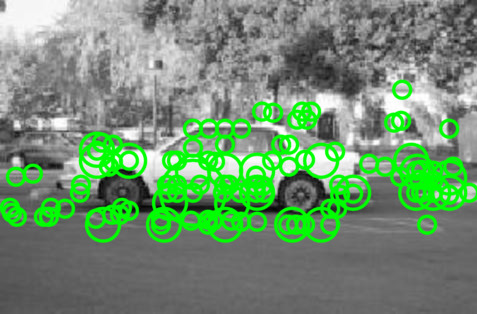
\includegraphics[width=0.49\linewidth]{images/fig5g.jpg}\label{fig:5g}}\hfil
\subfloat[Salient points]{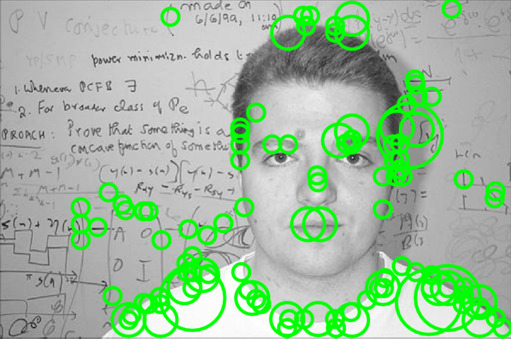
\includegraphics[width=0.49\linewidth]{images/fig5h.jpg}\label{fig:5h}}
\caption{Feature detection. (a)(d) Original images.
(b)(e) Complex cell activity map. 
(c)(f) Entropy map.
In the maps, red color indicates high value and blue color indicates low value.
(g)(h) Salient points at the scale of 4, 8, and 16 in terms of simple cell radius.}
\label{fig:5}
\end{figure}

\subsection{RBM encoders in V4 layer}

With saliency filters described in the previous subsection, we are able to focus on a limited number of salient points.
The V4 computation units in our model encode the shape in the neighborhood of each salient point.
The encoding is achieved with Restricted Boltzmann Machine (RBM).
RBM is widely used in unsupervised training of deep neural network \cite{bengio2009}.
\figurename~\ref{fig:6} shows such an RBM encoder in our model.
It encodes local shape features around a salient point, $(x,y)$.
For each preferred orientation, we select the complex cell of which the receptive field is centered at point $(x,y)$, and its eight neighbors.
\figurename~\ref{fig:6} demonstrates an example of three preferred orientations.
In this case, $9\times3$ complex cells are selected to form the input layer (or visible layer) of the RBM.
The output vector of the hidden layer forms a representation of local shape features.

\begin{figure}[!t]
\centerline{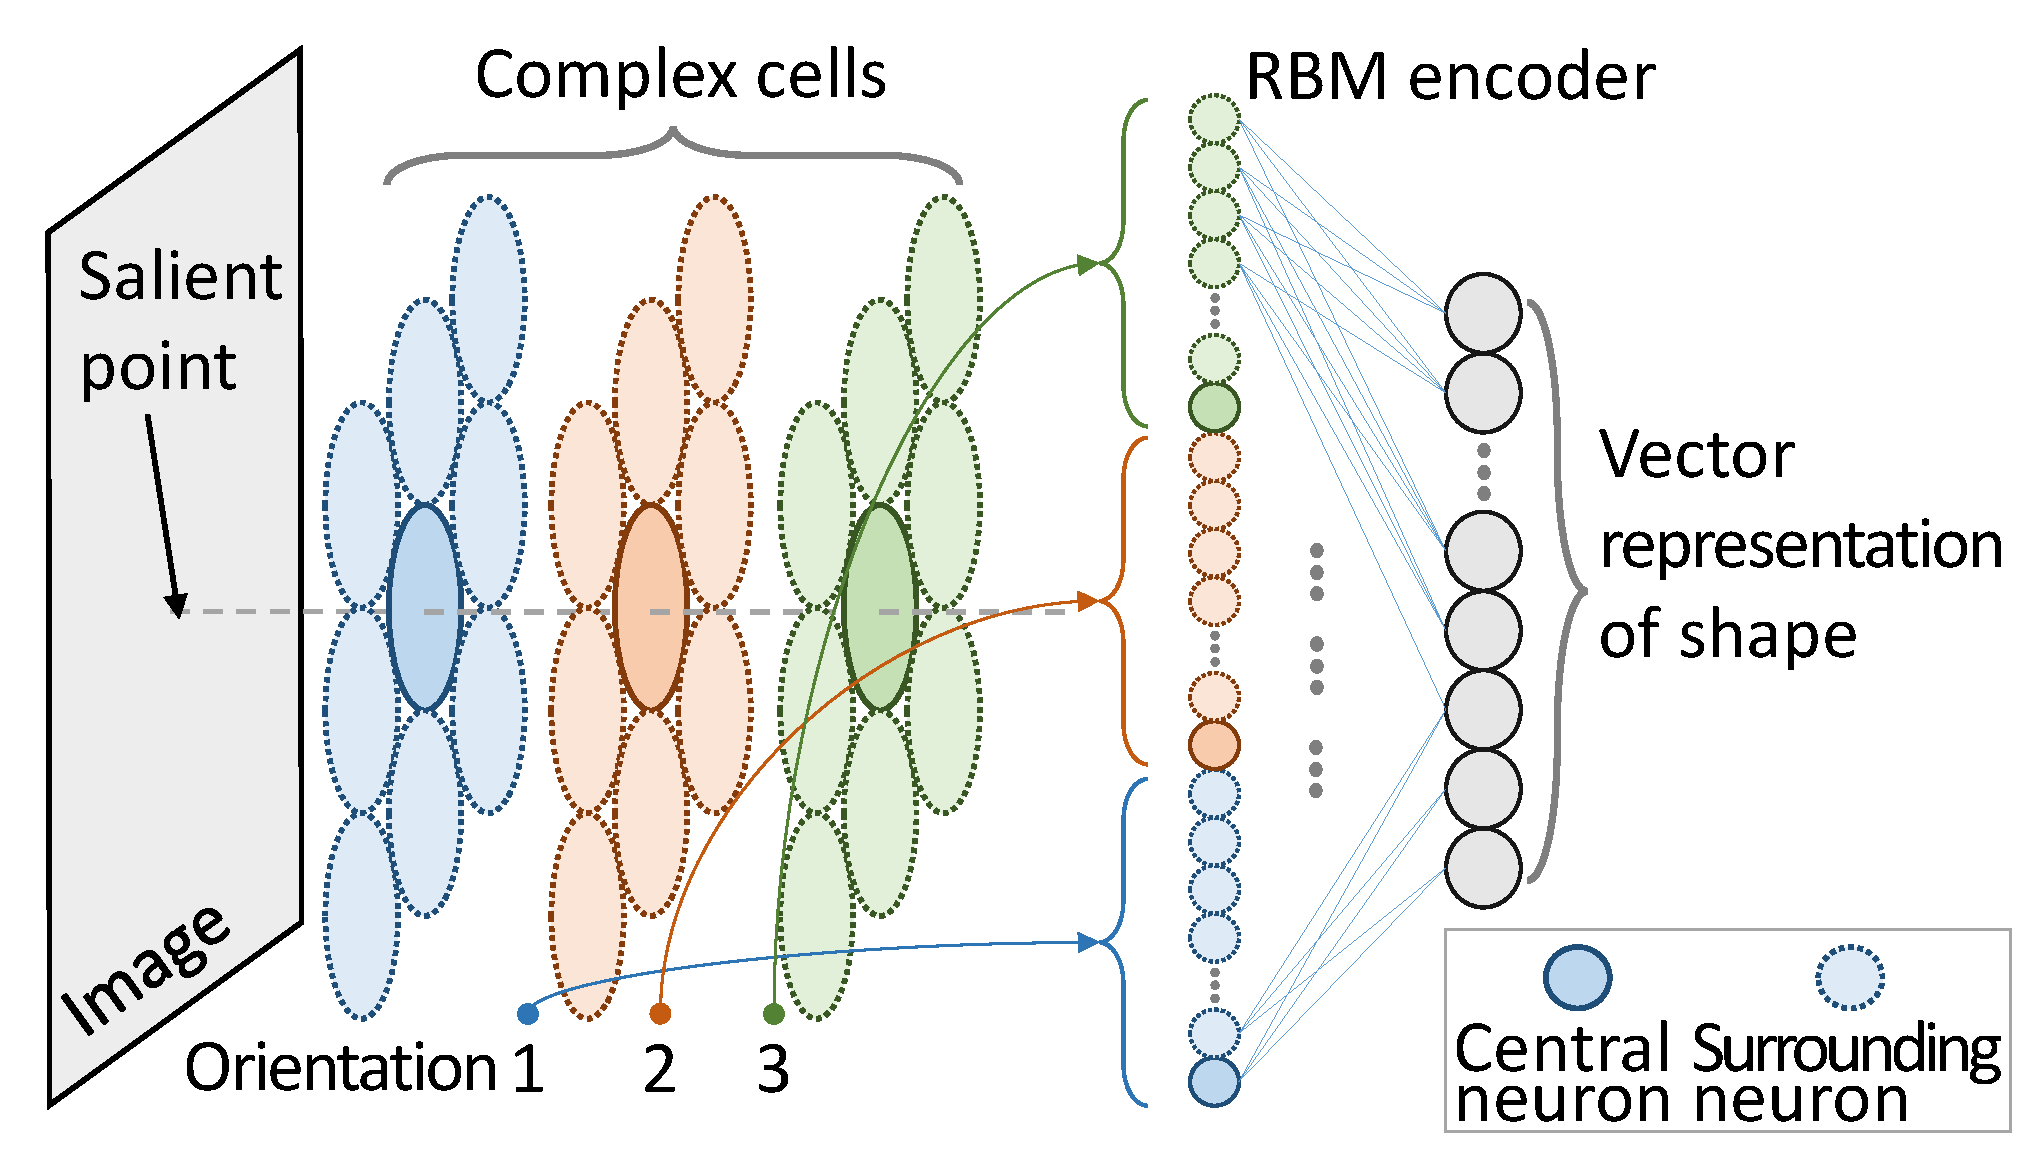
\includegraphics[width=0.99\linewidth]{images/fig6.eps}} 
\caption{RBM encoder for local shape feature.}
\label{fig:6}
\end{figure}

We followed \cite{hinton2010} for the training algorithm of RBM and the choice of parameters.
Weight-decay is used to reduce overfitting by adding an L2 penalty term, $\frac{1}{2}\lambda w^2$, to the energy function.
Let $w_{ij}$ be the connection weight between the $i$-th visible unit and the $j$-th hidden unit.
In each learning iteration, the change in the weight is given by
\begin{equation}
\Delta w_{ij}=\epsilon\left(\langle v_i h_j\rangle_\text{data}-\langle v_i h_j\rangle_\text{recon}\right)
-\epsilon\lambda w_{ij},
\end{equation}
where $\epsilon$ is the learning rate, $\lambda$ is the weight-cost coefficient,
$\langle v_i h_j\rangle_\text{data}$ is the product of two units when the visible layer is given real data,
and $\langle v_i h_j\rangle_\text{recon}$ is the product of two units when the visible layer is given reconstructed data.

\section{Experiments}\label{sec:4}

In this section, we demonstrate several experiments.
The first two experiments show that the shape selectivity of our model conforms to that of real V4 neurons.
The following experiments evaluate our model in feature matching and object recognition tasks.

\subsection{Perceptron over complex cells}

With this experiment, we demonstrate that artificial neurons which take input directly from complex cells can imitate neuronal response pattern of V4.
Therefore, it is feasible that we use a single layer of RBM to extract V4 features from complex cells.

In the experiment, a perceptron was configured to take complex cells as input.
It was then trained to distinguish between two shapes shown in \figurename~\ref{fig:7a}.
The shapes were also used to examine the selectivity of V4 in \cite{pasupathy2001}.
The difference between the two shapes is that one has a sharp corner towards the top right.

\begin{figure}[!t]
\centering
\subfloat[Response map]{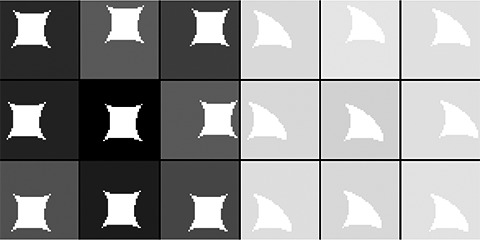
\includegraphics[width=0.48\linewidth]{images/fig7a.jpg}\label{fig:7a}}\hfil
\subfloat[Weight matrices]{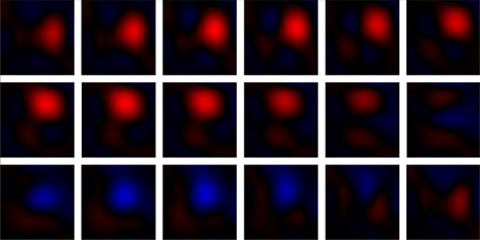
\includegraphics[width=0.48\linewidth]{images/fig7b.jpg}\label{fig:7b}}
\caption{Response map and weight matrices of a perceptron that distinguishes two shapes.
(a) Responses of the perceptron over 18 samples.
The perceptron prefers the shape in the left half of the samples.
It is insensitive to stimulus position.
(b) The input weight of the perceptron. 
Each block shows the weight of connections from complex cells of a certain orientation.
Complex cells of 18 different orientations provide input for this perceptron.}
\label{fig:7}
\end{figure}

Since V4 neurons show a certain degree of invariance in stimulus position,
we moved the shapes randomly within the receptive field of the perceptron 
to generate samples for training and testing (\figurename~\ref{fig:7a} shows several samples).
The samples were then used as input of the layers of simple cells and complex cells.
The output of complex cells were passed to the perceptron.
We had complex cells with 18 different preferred orientations (from $0^\circ$ to $170^\circ$ in steps of $10^\circ$) 
and over different positions in the V4 receptive field.
Therefore, the input of the perceptron consisted of 18 matrices, 
each corresponding to the output of complex cells with a certain orientation.
The input weight of the perceptron was thus also 18 matrices.

The trained perceptron exhibited a strong bias towards the shape with a sharp corner towards the top right.
It also showed a significant degree of invariance to the stimulus position.
It is obvious that this kind of selectivity is not formed from certain excitatory sub-regions
or inhibitory sub-regions of the receptive field which was found of simple cells \cite{hubel1962,pasupathy2001}.
The selectivity of the perceptron tallies with the selectivity of actual V4 neurons.
The response map is shown in \figurename~\ref{fig:7a}.
Darker background colors indicate stronger responses.
The input weight of this perceptron is shown in \figurename~\ref{fig:7b}.
Each block shows the weight from the complex cells of a certain preferred orientation.
Red color denotes positive weight while blue color denotes negative weight.

This experiment demonstrates that complex cells provide sufficient information for V4 neurons to show selectivity observed in neurobiological experiments.

\subsection{Shape selectivity}

In the following experiment, we trained our model to learn shapes.
After training, our model can distinguish the stimuli which V4 neurons are selectively tuned for.
The training samples were collected from \cite{gallant1996,pasupathy1999,pasupathy2001}, 
including 4 categories of stimuli, i.e., sinusoidal gratings, non-Cartesian gratings, segmented curves, and closed shapes.
The training process involved the layers of simple cells, complex cells and RBM encoders.
Since each sample image was fitted into a single V4 receptive field, the saliency filters were not involved in this experiment.

We used an RBM with 256 hidden units in this experiment.
In order to assess the selectivity of these units, we assigned each unit a selectivity index over a category of stimuli.
The selectivity index is defined as the ratio of the maximal response to the average response over the stimuli of a certain category.
Given an RBM output unit $h$ and its output value $h_i$ over the $i$-th stimulus in a category of $N$ stimuli.
The selectivity index $\mathcal{S}$ of $h$ is given by
\begin{equation}
\mathcal{S}(h)=\frac{\max\{h_i|i=1,2,\dots,N\}}{\sum_{i=1}^N h_i/N}.
\end{equation}
In the following statistics, we assumed that a unit has significant selectivity over a category of stimuli
if its selectivity index is greater than the average index.
Among the 256 units, 171 units exhibited significant selectivity for different stimuli.
102 units showed selectivity for segmented curves (\figurename~\ref{fig:8}).
55 units showed strong bias towards non-Cartesian gratings (\figurename~\ref{fig:9})
while 50 units showed selectivity for classical sinusoidal gratings.
68 units exhibited selectivity for closed shapes (\figurename~\ref{fig:10}).
The shape selectivity of our model is listed in \tablename~\ref{tab:1}.
The categories of selectivity are not mutually disjoint.
A single unit may possess more than one kind of selectivity simultaneously.

\begin{table}[h]
\caption{Shape selectivity of our model}
\centering
\begin{tabular}{|r|r|r|}
\hline
Selectivity & \#Units & Percentage \\\hline
Sinusoidal gratings & 50 & 19.5\% \\\hline
Non-Cartesian gratings & 55 & 21.5\% \\\hline
Segmented curves & 102 & 39.8\% \\\hline
Closed shapes & 68 & 26.6\% \\\hline
\end{tabular}
\label{tab:1}
\end{table}

\figurename~\ref{fig:8} show three response maps to segmented curves.
Darker background indicates stronger response.
It is shown that the three units exhibited strong bias towards curves rather than straight lines.
They were all tuned for the orientation of the projections.
This is compliant with the selectivity of V4 neurons described in \cite{pasupathy1999}.
\figurename~\ref{fig:9} shows the response maps of two units which are selective for non-Cartesian gratings.
Both of the two units were not sensitive to sinusoidal gratings.
\figurename~\ref{fig:10} shows the sample patterns of closed shapes and the response map of two units selectively tuned for two kinds of shapes.
They were sensitive to the angular position of the shapes \cite{pasupathy2001}.

\begin{figure}[!t]
\centering
\subfloat[]{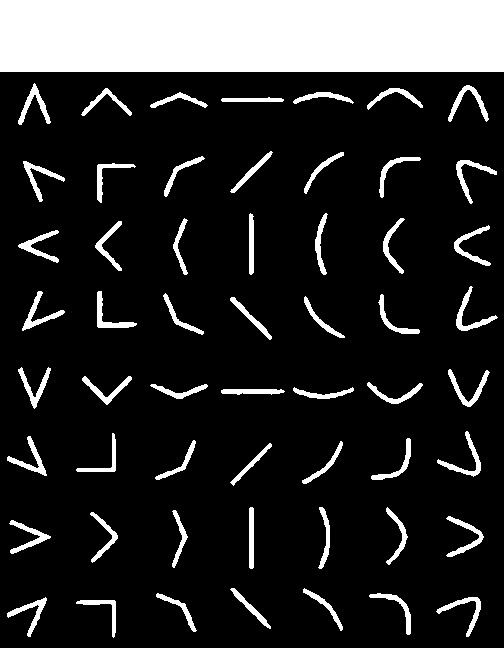
\includegraphics[width=0.24\linewidth]{images/fig8a.jpg}\label{fig:8a}}\hfil
\subfloat[]{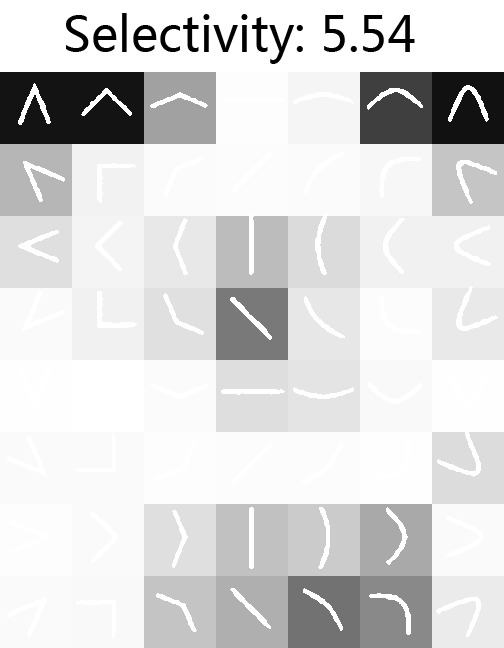
\includegraphics[width=0.24\linewidth]{images/fig8b.jpg}\label{fig:8b}}\hfil
\subfloat[]{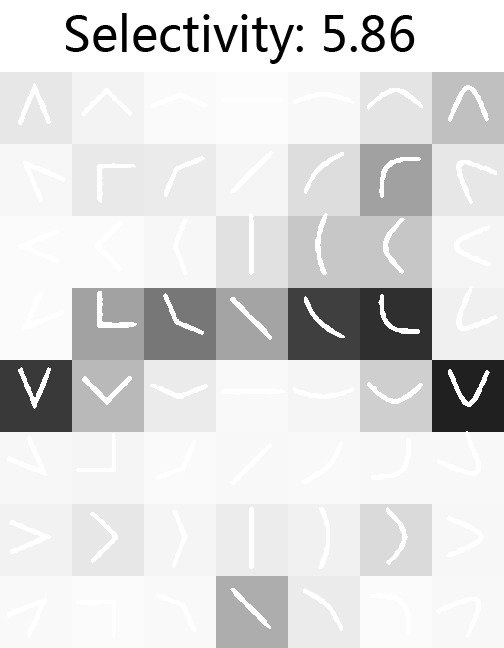
\includegraphics[width=0.24\linewidth]{images/fig8c.jpg}\label{fig:8c}}\hfil
\subfloat[]{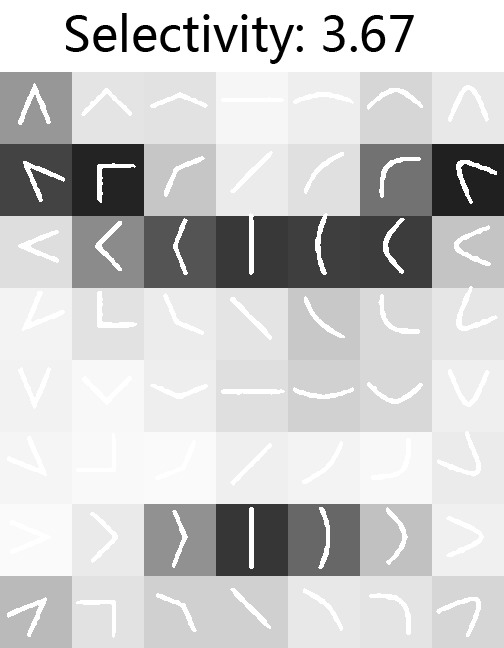
\includegraphics[width=0.24\linewidth]{images/fig8d.jpg}\label{fig:8d}}
\caption{RBM output units responding to convex curves towards certain directions.
(a) Sample patterns of segmented curves.
(b-d) Selectivity indexes and response maps of units tuned for upward, downward, and top-left projections. }
\label{fig:8}
\end{figure}

\begin{figure}[!t]
\centering
\subfloat[Response map of a unit selective for a pair of circular sectors (selectivity index = 3.92).]%
{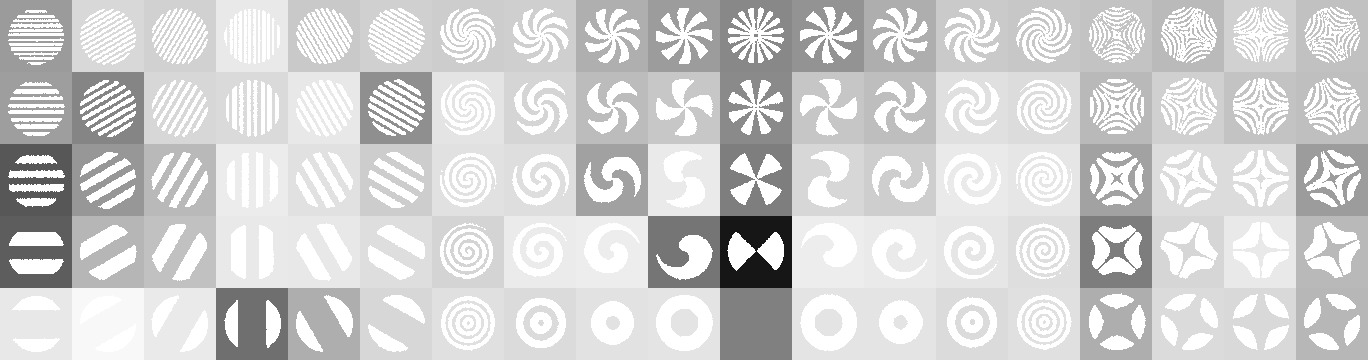
\includegraphics[width=0.9\linewidth]{images/fig9a.jpg}\label{fig:9a}}\\
\subfloat[Response map of a unit selective for helix shapes (Selectivity index = 6.37).]%
{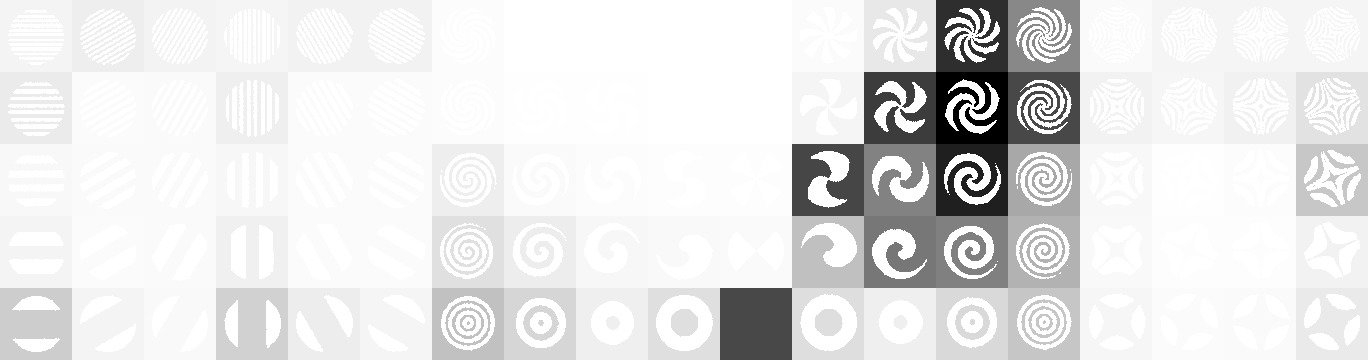
\includegraphics[width=0.9\linewidth]{images/fig9b.jpg}\label{fig:9b}}
\caption{Response maps of RBM units tuned for non-Cartesian gratings.}
\label{fig:9}
\end{figure}

\begin{figure}[!t]
\centering
\subfloat[Patterns]{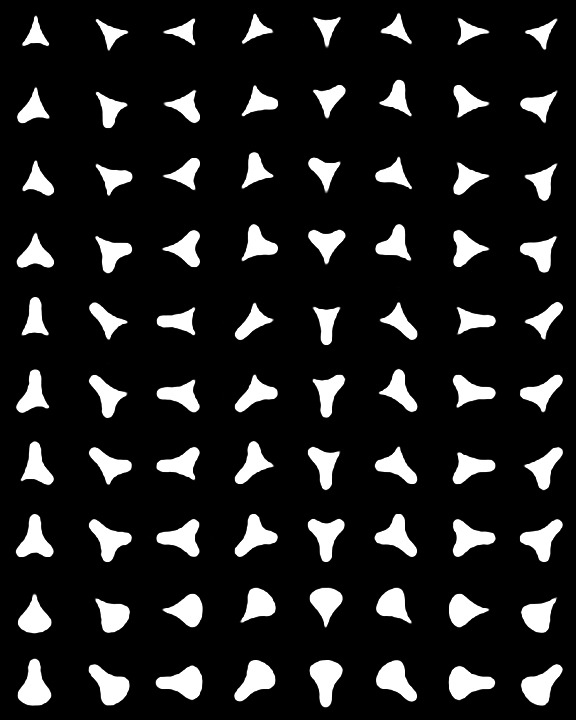
\includegraphics[width=0.31\linewidth]{images/fig10a.jpg}\label{fig:10a}}\hfil
\subfloat[Response map]{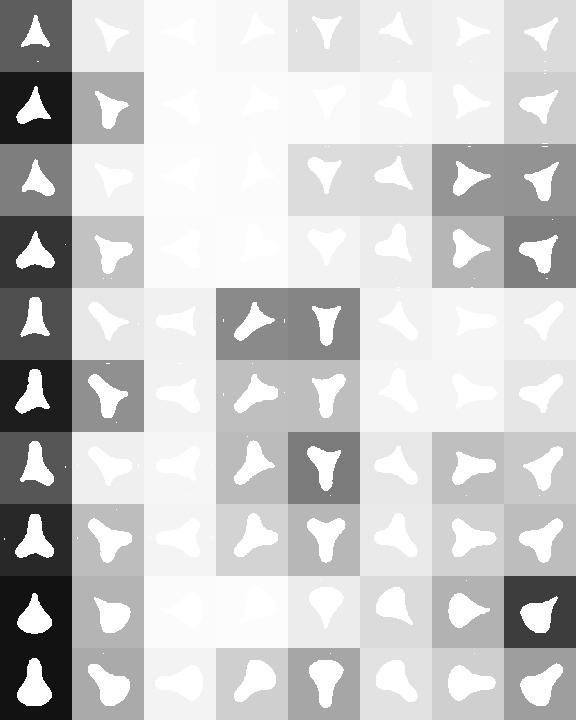
\includegraphics[width=0.31\linewidth]{images/fig10b.jpg}\label{fig:10b}}\hfil
\subfloat[Response map]{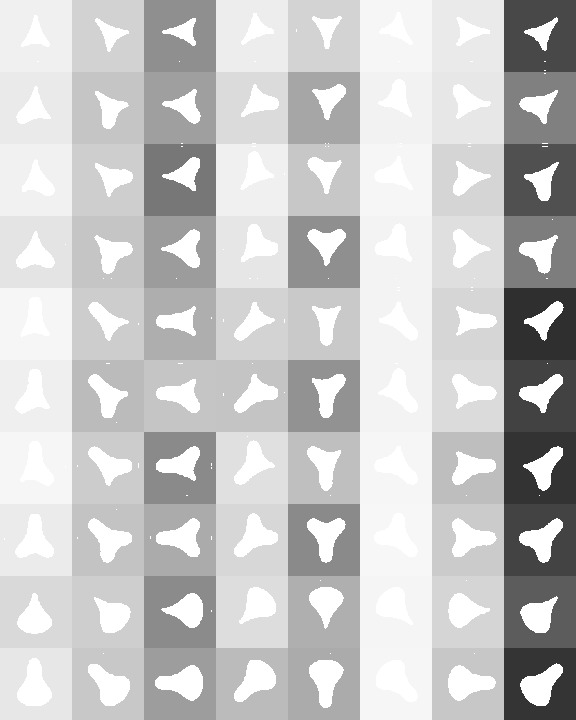
\includegraphics[width=0.31\linewidth]{images/fig10c.jpg}\label{fig:10c}}
\caption{RBM units responding to closed shapes.}
\label{fig:10}
\end{figure}

\subsection{Feature matching}

In this section, we demonstrate the performance of the features generated by our model in feature matching tasks.
We do not use typical criteria for evaluating local descriptors \cite{mikolajczyk2005}
for the reason that the typical criteria focus on matching the same physical point in different viewing conditions,
at which humans or other intelligent species are not significantly better than computer systems.
The human vision excels in image understanding tasks such as recognizing a new instance from some category.
It requires generalization ability of the features.

We first provide a qualitative evaluation.
The SIFT features \cite{lowe1999} are used for comparison.
The VLFeat open-source library \cite{vedaldi2010} were utilized for the SIFT implementation and the feature matching algorithm.

\begin{figure}[!t]
\centering
  \subfloat[Matching between the same face]{
    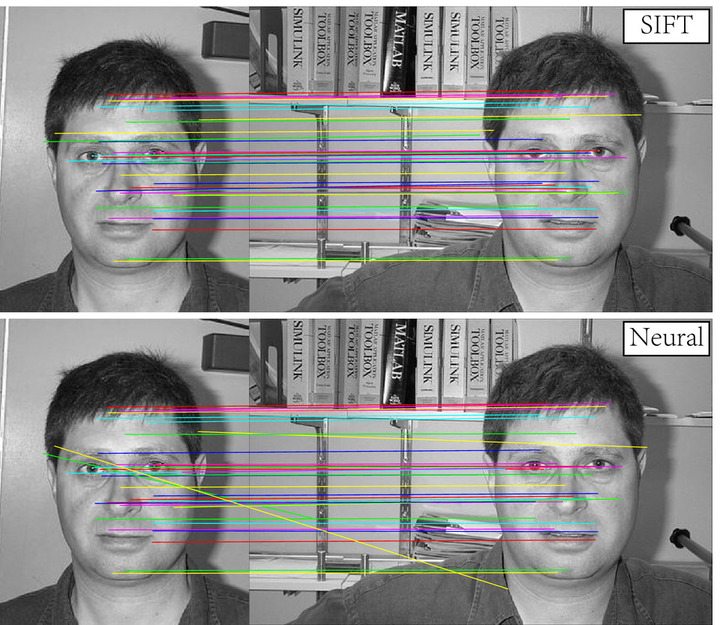
\includegraphics[width=0.8\linewidth]{images/fig11a.jpg}
    \label{fig:11a}}\\
  \subfloat[Matching between different faces]{
    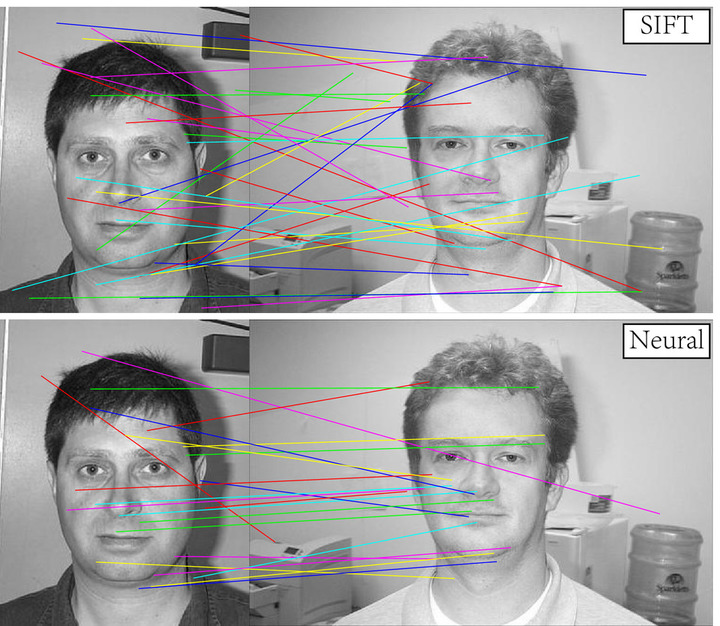
\includegraphics[width=0.8\linewidth]{images/fig11b.jpg}
    \label{fig:11b}}
\caption{Matching face images.}
\label{fig:11}
\end{figure}

\figurename~\ref{fig:11} shows matchings of features in face images.
As shown in \figurename~\ref{fig:11a}, both SIFT features and neural features match perfectly between face images of the same person.
However, \figurename~\ref{fig:11b} shows that matching of SIFT features between face images of different people is quite disordered.
SIFT features excel in matching highly distinctive features under image transformations
but lack the generalization ability to capture variations in objects appearance of the same category.
By contrast, the neural features show robust performance in matching features from different faces.
The result suggests that our model exhibits both competitive discrimination ability and better generalization ability compared with SIFT features.

\begin{figure}[!t]
\centering
  \subfloat[Our match]{
    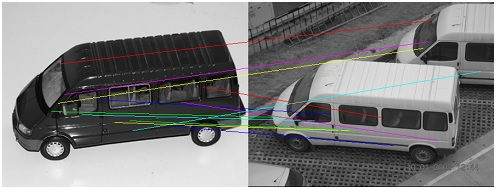
\includegraphics[width=0.8\linewidth]{images/fig12a.jpg}
    \label{fig:12a}}\\
  \subfloat[SIFT match]{
    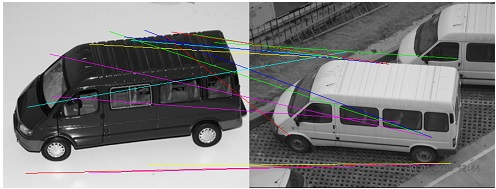
\includegraphics[width=0.8\linewidth]{images/fig12b.jpg}
    \label{fig:12b}}
\caption{Comparison of feature matching between van images.}
\label{fig:12}
\end{figure}

Another comparison in \figurename~\ref{fig:12} demonstrates
more clearly the advantage of our model compared with SIFT feature.
\figurename~\ref{fig:12a} shows that our model produced correct matches
between the model van in the left and the two real vans in the right. 
However, SIFT feature failed to produce correct matches (\figurename~\ref{fig:12b}). 
SIFT feature utilizes the direction of image gradient. 
It fails to capture the shape feature of an object when the object's color changes dramatically because the direction of image gradient changes with the color. 
Our model focuses on the shape feature and thus achieves a stable matching despite the change in color.

For quantitative evaluation, we use the ``Face-easy'' category from the Caltech 101 dataset \cite{fei2007}.
This category consists of frontal face photos of many different people.
They are all cropped to the same size and the same face location.
The images are randomly paired for feature matching.
A correct match between facial features should be corresponding regions in the two images.
We use precision-recall curves to compare our neural features with the SIFT features.
\begin{equation}
\text{Precision} = \frac{\text{\#correct matches}}{\text{\#correct matches} + \text{\#false matches}}.
\end{equation}
\begin{equation}
\text{Recall} = \frac{\text{\#correct matches}}{\text{\#all features}}.
\end{equation}
The result is shown in \figurename~\ref{fig:13}.
Extensive evaluation on the generalization ability of our features is in the object recognition experiment in the next subsection.

\begin{figure}[!t]
\centerline{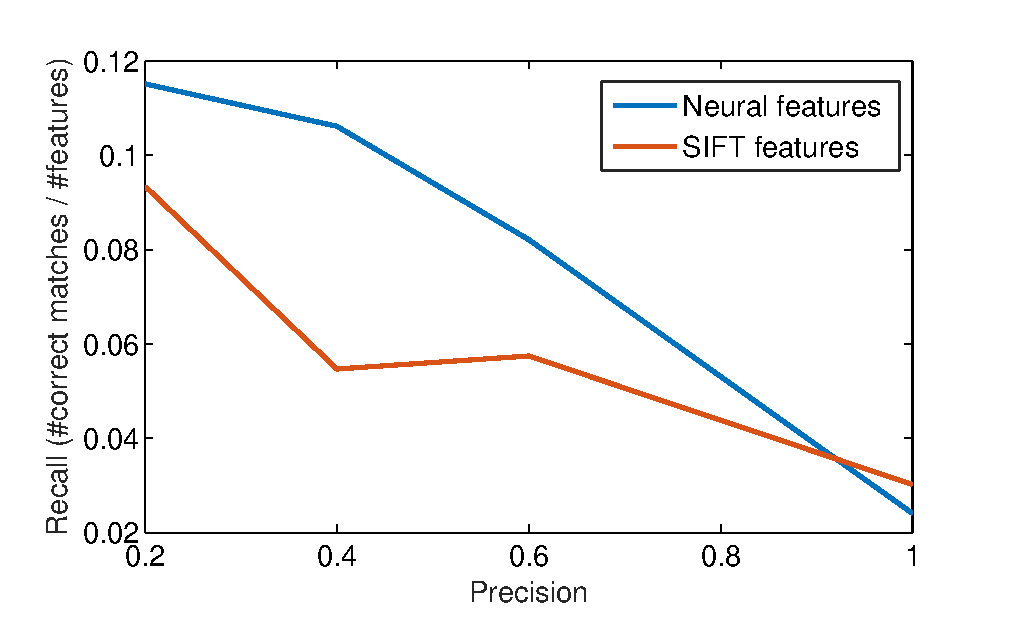
\includegraphics[width=0.9\linewidth]{images/fig13.eps}} 
\caption{Matching facial features in Caltech-101 ``Face-easy'' category.}
\label{fig:13}
\end{figure}

\subsection{Object recognition}

We evaluate the performance of the proposed model in object recognition in clutter for which 
the target object in both the training and test samples appears at variable scales and positions within an unsegmented image.
Features at the salient-points are extracted and passed to a classifier.
We experimented with the SVM classifier and evaluated the classifier over the Caltech 101 dataset \cite{fei2007}.

In the RBM encoders of V4 units, the visible RBM units collect their input from complex cells with different preferred orientations.
Therefore, we investigate the selection of sampling density of orientations (i.e., the number of different preferred orientations).
The result is shown in \figurename~\ref{fig:14a}.
In this experiment, 30 training samples are randomly chosen from each category.
For each training image, 50 features are randomly chosen and passed to the classifier.
The result shows that selection of sampling density does not exhibit obvious impact on the performance.
With a small density, we can lower the dimension of the input of RBM encoders without a significant loss in object recognition performance.
Thus in the succeeding experiments, a sampling density of $3$ is used. 

\begin{figure}[!t]
\centering
  \subfloat[Sampling density of orientations]{
    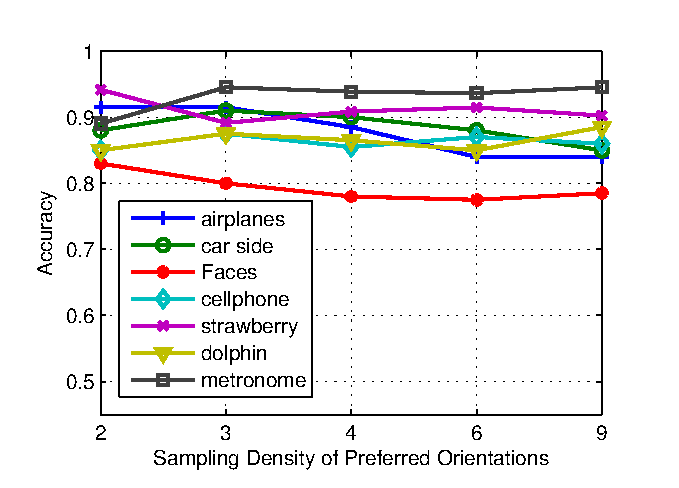
\includegraphics[width=0.9\linewidth]{images/fig14a.eps}
    \label{fig:14a}}\\
  \subfloat[Number of features per image]{
    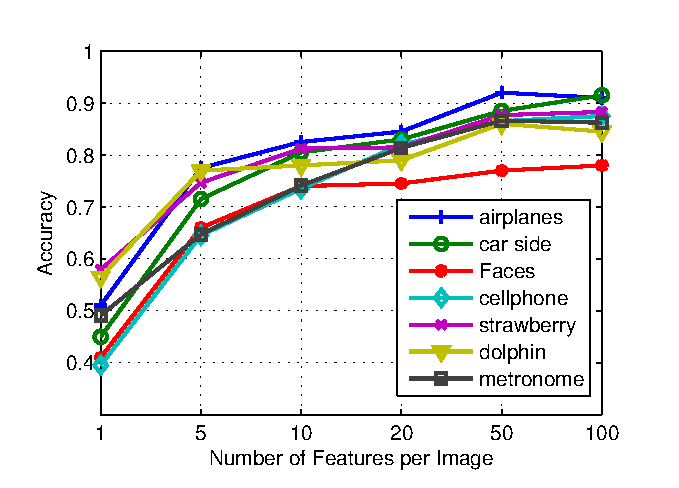
\includegraphics[width=0.9\linewidth]{images/fig14b.eps}
    \label{fig:14b}}
\caption{Performance with different parameters.}
\label{fig:14}
\end{figure}

We can also control the number of features extracted from an image by adjusting the threshold in the saliency filters. 
To investigate the contribution of the number of features on performance, we vary the number of features chosen from each training image.
We choose 20 training samples from each category.
The result is shown in \figurename~\ref{fig:14b}.
With 50 features per image the result approaches the best performance.
In the succeeding experiments, we take 50 features from each image.

The influence of the number of training samples on the performance of our model is also studied.
For each category, we randomly select training sets of size 5,10,15,20,25 and 30.
\figurename~\ref{fig:15a} shows the performance as a function of the number of training images.
The results reported are averaged over all categories.
The performance is compared with other published results \cite{grauman2005,lazebnik2006,zhang2006,wang2006,bosch2007,boiman2008,liu2013,heo2014}.

\begin{figure}[!t]
\centering
  \subfloat[Comparison with other methods]{
    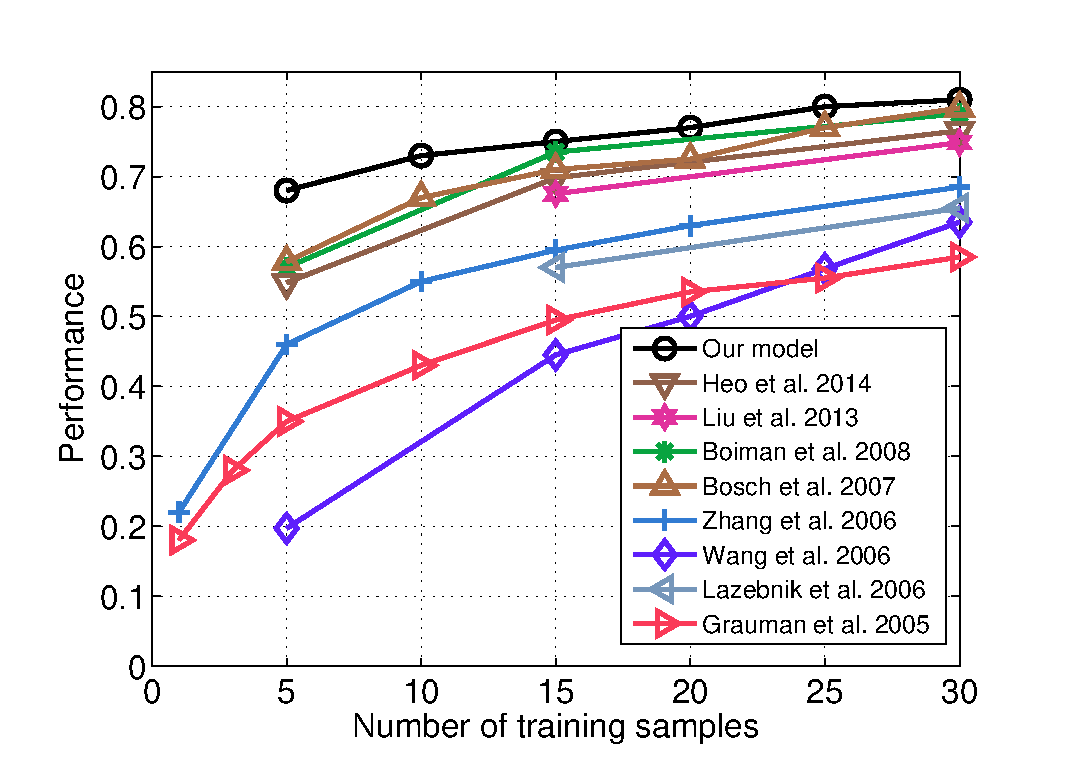
\includegraphics[width=0.9\linewidth]{images/fig15a.eps}
    \label{fig:15a}}\\
  \subfloat[Comparison with other features]{
    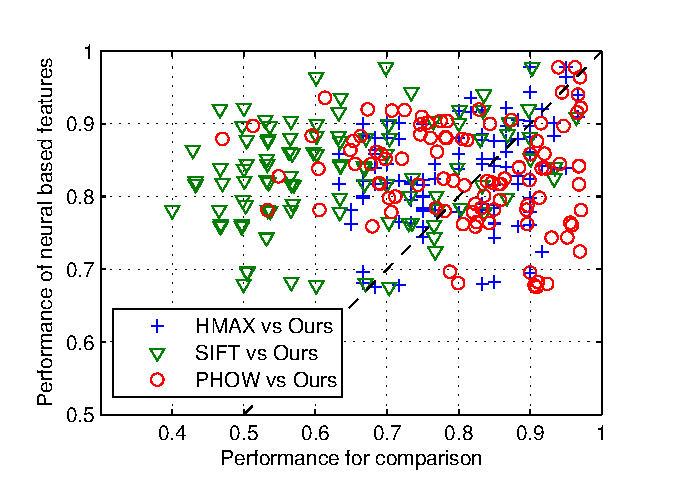
\includegraphics[width=0.9\linewidth]{images/fig15b.eps}
    \label{fig:15b}}
\caption{Comparison of performance.}
\label{fig:15}
\end{figure}

\figurename~\ref{fig:15b} shows the performance of our model over the 101 categories
compared with SIFT features \cite{lowe1999}, PHOW features \cite{lazebnik2006}, and biologically inspired HMAX model \cite{cadieu2007}.
The results are obtained with 30 training images randomly selected from each category.
Our model exhibits competitive performance compared with other models.
As shown in \figurename~\ref{fig:15b}, the SIFT performance points over the 101 categories are almost completely to the left of the equivalent line.
The PHOW performance points spread through a wider range from $0.5$ to $1$ indicating the lack of robustness compared with our model.
Compared with the biologically inspired HMAX model, our performance is also better for more than half of the 101 categories.

\section{Discussion and conclusion}\label{sec:5}

\begin{table*}[!t]
\caption{Comparison of different models}
\centering
\small
\begin{tabular}{|p{0.15\linewidth}|p{0.22\linewidth}|p{0.22\linewidth}|p{0.22\linewidth}|}
\hline
& Our model & HMAX & Deep learning \\\hline
Number of layers & 3 & 2 & $2\sim8$ \\
& ($+$ saliency filters) & ($+2$ pooling layers) & ($+2\sim3$ pooling layers)\\\hline
Input images & various size & various size & fixed size \\
& (multi-scale salient point detector) & (full-scan with fixed-size window) & \\\hline
Training samples & $5\sim50$ & $5\sim50$ & $>10^4$ \\
& (per category) & (per category) & (for unsupervised pre-training) \\\hline
Training & restricted Boltzmann & greedy search for fitting & restricted Boltzmann \\
algorithms & machine (only V4 layer) & V4 neuron; radial basis function network for image feature extraction & machine (all layers) \\\hline
\end{tabular}
\label{tab:2}
\end{table*}

The model proposed in this paper is a biologically motivated model for shape-based image feature extraction.
Traditional image descriptors utilize flat models which extract features directly from the image via statistical or algebraic techniques \cite{mikolajczyk2005}. 
On the contrary, our proposed model simulates the biological vision in the level of neural mechanism.
Its multilayer structure resembles the neural systems and extracts information from simple features to gradually more complex features. 

Previous work on biologically inspired models shows that efficient object recognition algorithms can be developed 
based on the representation generated by the primary visual cortex \cite{wei2014,wei2014b,zhao2013}.
In this paper, we investigate deeper into higher levels of the visual cortex.
We simulate the shape selectivity in area V4 because the shape or contour of an object is generally stable and invariant, which provides a good basis for recognition.

The HMAX model \cite{cadieu2007} and the deep learning model \cite{bengio2009}, which both draw inspiration from the neural systems, 
construct similar multilayer structures.
In particular, the deep model exhibits high performance in classifying very large image database \cite{krizhevsky2012}.
However, a deep model is a neural network of very large scale (In \cite{krizhevsky2012}, the network has 8 layers and more than 400,000 neurons),
and training such a model generally requires a large number of training samples (\cite{krizhevsky2012} uses 1.2 million training images).
Deep learning is a process of fully automatic feature extraction.
Limited training samples can not provide enough variety to keep the model from over-fitting.
The HMAX model consists of fewer layers and only one layer (S2 layer) is trainable, which allows the model to work on limited training samples.
In the proposed model, we combine these two approaches.
The layers corresponding to the primary visual cortex is artificially designed with prior knowledge of the cortical neurons.
V4 features are automatically extracted based on the output of the artificially designed network.
This strategy saves us from retraining the first layers every time.
Additionally, we implement a layer of saliency filters to detect key-points in images,
which enables the model to process images of various sizes efficiently. 
In \tablename~\ref{tab:2}, we summarize the comparison of the three models.

Future work should involve further investigation into the visual systems and extensive evaluation on shape-based object detection.

\bibliographystyle{unsrt}
\bibliography{ref}

\end{document}